\section{Introduction}
\label{sec:intro}

Camera-based tactile sensors such as GelSight~\cite{yuan2017gelsight,dong2017improved} and DIGIT~\cite{lambeta2020digit} render contact as an image: an elastomer gel is pressed against a surface, and internal LEDs shade its deformation for a camera. Learned perception on these images now covers material identity, force, slip and pose, and tactile foundation models pretrained on millions of frames are available~\cite{higuera2024sparsh,t3fota2024,anytouch2025}. Almost all of it is developed and evaluated inside short recording campaigns. In a robot hand, the same sensor touches objects for weeks: it is powered up and down, its gel is lubricated, worn and eventually replaced. Whether a representation learned in June still works in October is, to our knowledge, untested: no public tactile dataset holds out a later session of the same sensor unit, and the closest proxies swap units or gels~\cite{sitr2025,tacverse2026,bideta2026}.

\begin{figure}[t]
  \centering
  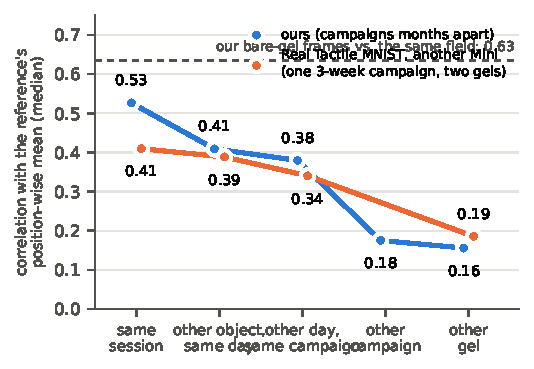
\includegraphics[width=\linewidth]{fig/fig_day_signature.pdf}
  \caption{\textbf{Contact images carry a day signature of the sensor.} Median correlation between the fine band (190--370\,\si{\micro\metre}) of a contact image and the position-wise mean of other contacts, as a function of how the reference relates to the contact. On our sensor (blue, 55 sessions over four months) a contact matches other \emph{objects} touched the same day almost as well as other contacts of its own session, and barely matches another day or the other gel. The same ordering appears on another lab's GelSight Mini (orange, Real Tactile MNIST~\cite{tactilemnist2025}, 24 runs over 15 days). Our no-contact frames do not contain the pattern (dashed).}
  \label{fig:signature}
\end{figure}

We recorded 2{,}711 grasps of 20 materials with one GelSight Mini over four months, in four campaigns separated by weeks, with the normal force co-recorded by a force sensor on the opposing finger, and, in the last campaign, bare-gel frames before and between grasps. Holding out the last campaign reveals a failure that no cross-unit study predicts. A supervised encoder trained in June--July recognises materials in September--October at \SupFoneRawSAcc\pct\ (chance 5\pct) and assigns \SupFoneRawSTop\pct\ of all episodes to a single class; frozen Sparsh encoders~\cite{higuera2024sparsh}, pretrained on GelSight Mini data, do no better (\SdinoRawAcc--\IjepaRawAcc\pct).

The cause is measurable without any model (\cref{fig:signature}). At a fixed image position, the fine-scale content of a contact image correlates with the average of \emph{other objects touched the same day} at \SigSameDay\ (median over sessions), almost as much as with the same session's other contacts (\SigOwn), and only at \SigOtherEra\ with another day's. The pattern is broadband, is strongest on rigid samples that cannot transmit a backing, and is \emph{absent from no-contact frames} (\num{0.06}): it is a property of the loaded gel on that day. Because a recording session holds one object, any material classifier can satisfy its labels with the day signature, and does; an era classifier applied to June contacts re-rendered under a July sensor state calls them July (\cref{sec:signature}).

This paper makes four contributions.
\textbf{(1)} We measure the day signature and its drift mechanisms---slow with use, a step at every power-up, a reset at gel replacement---on 620 bare-gel frames and 55 sessions, and replicate the signature on a second unit in public data.
\textbf{(2)} We show that the signature is the shortcut: every encoder we test collapses on a later day, and the standard fix, batch-norm re-estimation per session, collapses to chance because a session holds one object; on a public dataset whose runs hold all objects it works, confirming the mechanism.
\textbf{(3)} We separate sensor state from touch using only the robot's own contact stream. The \emph{loaded state}, the position-wise mean of recent contacts, is subtracted at test time (every encoder recovers: frozen Sparsh \num{3}$\times$, a supervised CNN \SupFoneRawSAcc$\rightarrow$\SupFonePrevSAcc\pct, and \SupAugFonePrevSAcc\pct\ with standard photometric jitter) or used at training time: re-rendering training contacts under other sessions' states and contrasting against position-matched decoys trains, with no labels and no test-time data, a small adapter that lifts frozen Sparsh-I-JEPA from \IjepaRawAcc\ to \IjepaAdAcc\pct.
\textbf{(4)} We show which cues survive: normal force read as marker spreading against the \emph{unloaded} gel transfers across months ($r$=\ForceGeomXeraC), where every appearance-based force estimate fails ($R^2\le\ForceLearnedBestR$); contact detection needs the same unloaded reference. The picture that emerges is a state-aware decomposition rather than one more invariant network: appearance needs the loaded state removed, geometry needs the unloaded state, and both states come from the stream the robot already produces.
